Das Brettspiel ist unter Verwendung von \acf{HTML5} und JavaScript-Modulen entwickelt. Zum Datenaustausch wird der vom Peer-Objekt bereitgestellte Datenkanal verwendet. Jeder Spieler besitzt eine eigene Kopie des Spielstands, welcher zwischen den Peers synchron gehalten werden muss. Zu diesem Spielstand gehören die in Abbildung~\ref{lst:spielstand} aufgelisteten Parameter, mit zugehörigen Standartwerten bei Initialisierung des Spiels.

\vspace{5pt}
\lstset{language=js, style=STYLE_CODE_JS}
\begin{minipage}{\textwidth}
\begin{singlespace}
\begin{lstlisting}[caption={Spielstandsdaten -- Game.js}, captionpos=b, label={lst:spielstand}]
export default function Game([...]) {
  [...]
  this.gamestate = {
    fsm : 'start',       // Zustand des Spiels (start|roll|move|end)
    pieces : [],         // Positionen der Spielfiguren
    current : -1,        // Farbe des Spielers am Zug
    lastRoll : -1,       // Zuletzt geworfene Zahl
    currentRolls : -1,   // Anzahl an Wuerfen im momentanen Zug
    canRollAgain : false // Kann der Spieler am Zug erneut wuerfeln?
  };
  [...]
}
\end{lstlisting}
\end{singlespace}
\end{minipage}

\subsubsection{Synchronisation des Spielstands bei Spielbeitritt}
Ist das Spiel gestartet, so weicht der Spielstand von den in Abbildung~\ref{lst:spielstand} gelisteten Standartwerten ab. In diesem Fall muss ein neu beitretender Spieler den gesamten Spielstand von einem weiteren Spieler zugeschickt bekommen. Dies wird immer vom Host des Spielraums übernommen, wenn der Datenkanal zum neuen Spieler geöffnet ist (vgl. Quellcode~\ref{lst:sendspielstand}). Dazu wird das \textit{gamestate}-Event verwendet.

\vspace{5pt}
\lstset{language=js, style=STYLE_CODE_JS}
\begin{minipage}{\textwidth}
\begin{singlespace}
\begin{lstlisting}[caption={Senden des Spielstands -- game.js}, captionpos=b, label={lst:sendspielstand}]
// aufgerufen wenn alle (neuen) Datenkanaele offen sind
peer.on('dataChannelsOpen', () => {
  if (isHost && game.gamestate.fsm !== 'start') {
    peer.emit(peerID, 'gamestate', game.gamestate);
  }
  [...]
});
\end{lstlisting}
\end{singlespace}
\end{minipage}

Auf der Empfängerseite muss der Spielstand entsprechend aktualisiert, und die Figuren an deren jeweiligen Positionen bewegt werden.

\subsection{Spielablauf}
\begin{figure}[h]
\centering
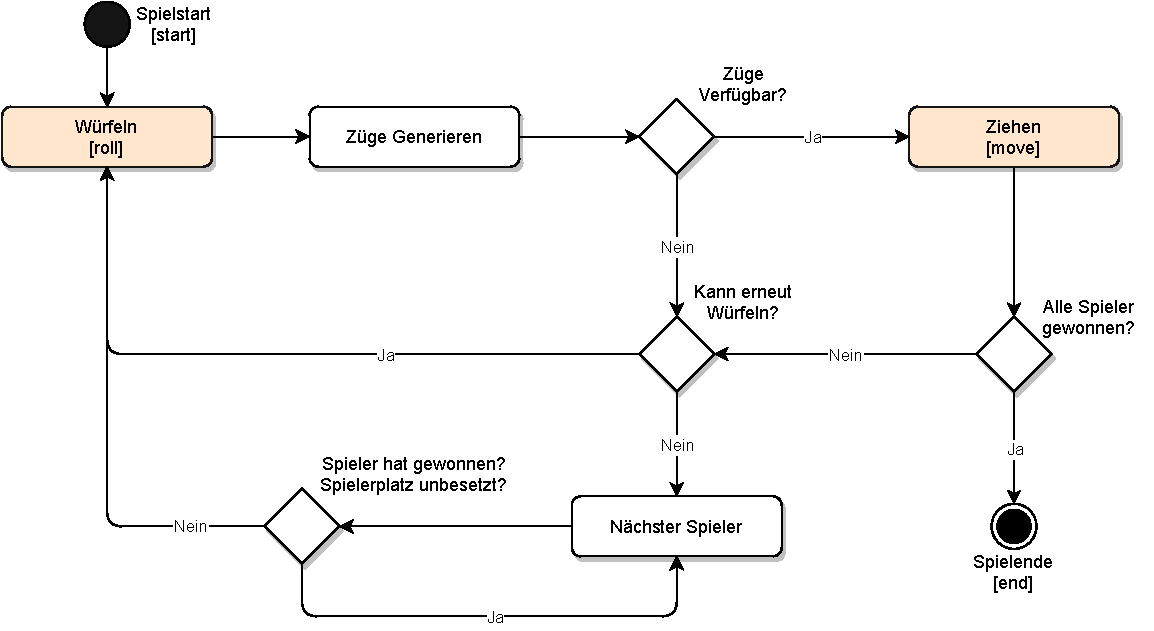
\includegraphics[width=0.95\textwidth]{bilder/PDF_SVG/MAEDN_ABLAUF.pdf}
\caption{Ablaufdiagramm des Brettspiels.}
\label{fig:maednablauf}
\end{figure}

Das Spiel lässt sich als Zustandsmaschine modellieren. Ein vereinfachtes Ablaufdiagramm des Spielverlaufs ist in Abbildung~\ref{fig:maednablauf} dargestellt. Die \glqq{}Zustände\grqq{} sind dabei in eckigen Klammern definiert. \textit{Kann erneut Würfeln} ist keine einzelne Kondition, sondern eine Ansammlung verschiedener Konditionen: Ein Spieler kann erneut würfeln, falls sich alle dessen Figuren in den A-Feldern befinden, und dieser in diesem Zug unter drei mal gewürfelt hat. Ein Spieler darf zudem immer neu würfeln, falls dieser eine sechs geworfen hat.

Die in orange hervorgehobenen Zustände \glqq{}Würfeln\grqq{} und \glqq{}Ziehen\grqq{} sind von besonderer Bedeutung, da an diesen Punkten ein Datenaustausch zwischen Spielern notwendig ist. Die ausgeführte Logik unterscheidet sich hier basierend darauf, ob ein Spieler am Zug ist oder nicht.\par

\subsubsection{Würfeln}
JavaScript bietet standartmäßig keine Möglichkeit, einen \textit{Seeded-Random-Number-Generator} zu erstellen. Aus diesem Grund wird die \glqq{}seedrandom\grqq{}-Bibliothek eingebunden\footnote{seedrandom: \url{https://github.com/davidbau/seedrandom}, Stand 12.05.2021}. Die Bibliothek stellt die \textit{Math.seedrandom}-Funktion bereit, welche einen Pseudozufallszahl-Generator erstellt. Standartmäßig nutzt dieser die Stromverschlüsselung \acf{RC4} zum Generieren von Zufallszahlen \cite{seedrandom}.

\vspace{6pt}
\begin{figure}[h]
\centering
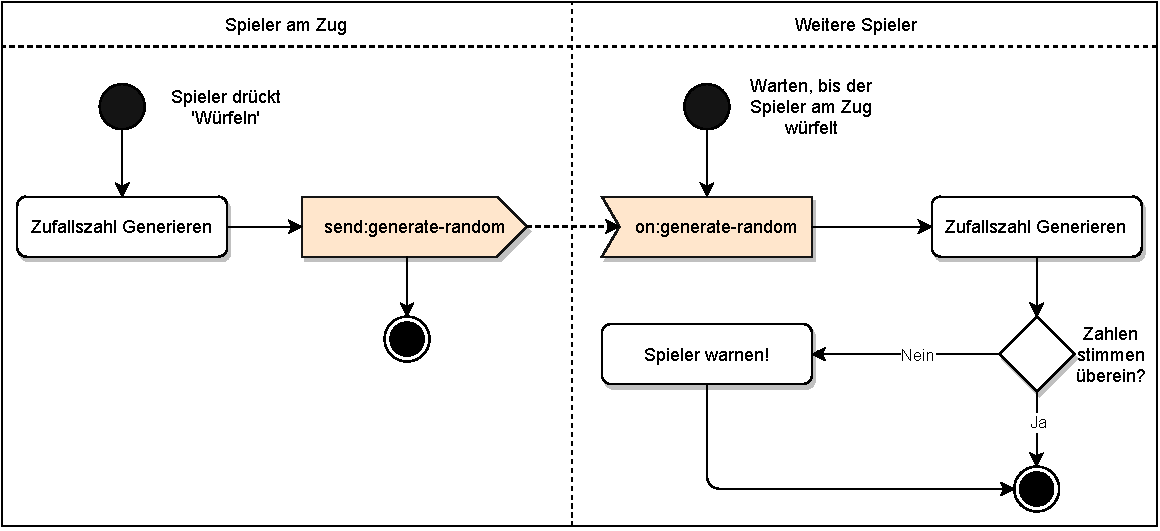
\includegraphics[width=0.90\textwidth]{bilder/PDF_SVG/MAEDN_WUERFELN.pdf}
\caption{Würfel-Nachrichtenaustausch.}
\label{fig:maednwuerfeln}
\end{figure}

Würfelt ein Spieler, so wird über den \textit{Seeded-Random-Number-Generator} eine Pseudozufallszahl generiert. Damit die Zufallszahlgeneratoren der weiteren Spieler synchron sind, muss diese Aktion den weiteren Spielern mitgeteilt werden. Dazu wird das \textit{generate-random}-Event an alle weiteren Peers gesendet. Die Parameter dieses Events enthalten die Zufallszahl des Spielers am Zug. Erhält ein weiterer Spieler das Event, so generiert dieser eine eigene Zufallszahl, welche -- falls der Spieler am Zug nicht betrügt, und die Zufallszahlgeneratoren der Spieler synchron sind -- gleich der vom Spieler am Zug generierten Zufallszahl sein sollte (vgl. Abbildung~\ref{fig:maednwuerfeln}).\par 

Mit der gewürfelten Zahl wird daraufhin ein Array mit allen möglichen Spielzügen generiert, welche der Spieler am Zug basierend auf der gewürfelten Zahl ausführen kann. Ein Zug setzt sich aus einer Start- und Zielposition zusammen:

\lstset{style=STYLE_COMMAND_LINE_ARGUMENT_SINGLE_LINE}
\begin{minipage}{\textwidth}
\begin{singlespace}
\begin{lstlisting}[belowskip=-0.8 \baselineskip]
move = {
  from : <relative-position>,
  to : <relative-position>
}
\end{lstlisting}
\end{singlespace}
\end{minipage}
\vspace{5pt}

Die Start- und Zielposition eines Zugs ist dabei immer relativ zum Start-Feld des Spielers am Zug. Sowohl der Spieler am Zug, als auch alle weiteren Spieler generieren das Array an Spielzügen.\par

\subsubsection{Ziehen}
Der Spieler am Zug kann durch Klicken auf eine Spielfigur einen Zug wählen. Existiert dieser im Zug-Array, so wird der gewählte Zug den weiteren Spielern per Event über die \acs{P2P}-Verbindung mitgeteilt. Die weiteren Spieler prüfen, ob dieser Zug in deren eigenen Zug-Arrays existiert. Existiert der Zug nicht, so wird davon ausgegangen, dass der Spieler am Zug betrügt, und eine Warnung wird ausgegeben. Hier unterscheidet sich die Logik also wieder zwischen dem Spieler am Zug und weiteren Spielern (vgl. Abbildung~\ref{fig:maednziehen}).

\vspace{6pt}
\begin{figure}[h]
\centering
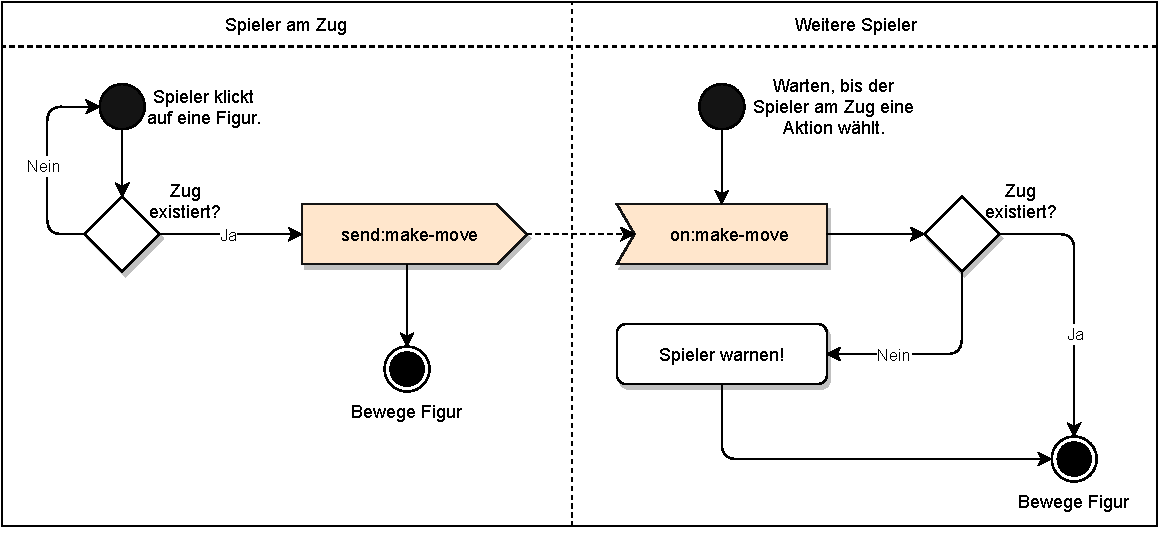
\includegraphics[width=0.90\textwidth]{bilder/PDF_SVG/MAEDN_ZIEHEN.pdf}
\caption{Ziehen-Nachrichtenaustausch.}
\label{fig:maednziehen}
\end{figure}

\subsection{Darstellung des Spielbretts}
Das Spielbrett wird aus stilisierten \acf{DOM}-Elementen generiert. Diese Elemente werden auf einem 11x11-Raster positioniert (vgl. Abbildung~\ref{fig:maednbrett}). Bei den Spielfiguren handelt es sich ebenfalls um \acs{DOM}-Elemente, welche dynamisch, basierend auf dem Spielstand, an verschiedene Feld-Elemente angefügt werden. Um die Spiellogik universell für jeden Spieler anwenden zu können, besitzen die Spielerspezifischen A- und B-Felder \glqq{}relative\grqq{} Positionen (\textit{<Farb-ID>:<Position>}). Diese Positionen sind relativ zu dem Start-Feld der jeweiligen Spielerfarbe. Die \glqq{}weißen\grqq{} Felder (0-39) besitzen lediglich eine \glqq{}absolute\grqq{} Position. Das letztendlich generierte Spielbrett ist in Abbildung~\ref{fig:maedngame} dargestellt.\par

\begin{figure}[h]
\centering
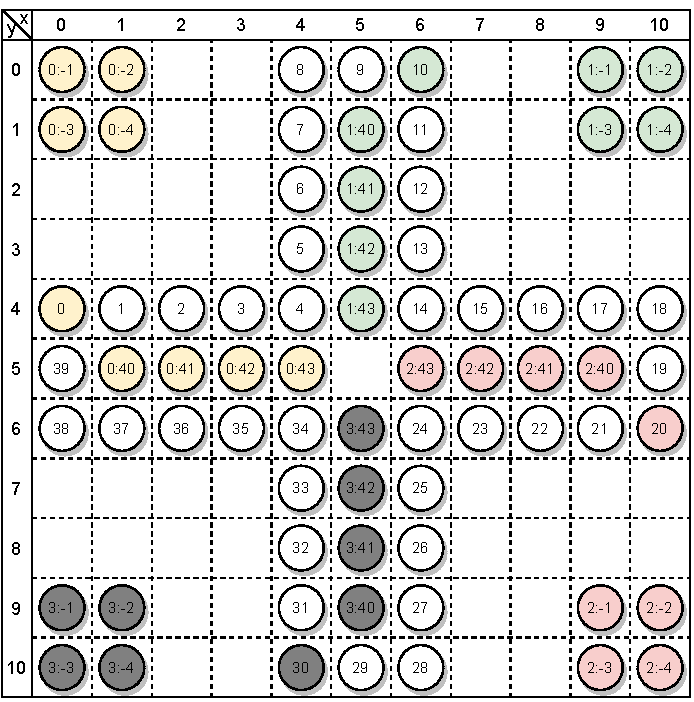
\includegraphics[width=0.90\textwidth]{bilder/PDF_SVG/MAEDN_BOARD_DIAGRAM.pdf}
\caption{Schemenhafte Darstellung des Spielbretts, mit Positionen und Farben.}
\label{fig:maednbrett}
\end{figure}
